\section{Related Works}
\label{se:related_work}
\subsection{Draft Model Design}
Numerous studies have explored the design of better draft models for speculative decoding. In principle, any autoregressive probabilistic model can serve as a draft model. The simplest approaches include using n-gram models \citep{ou2024lossless} or document retrieval as draft models \citep{yang2023inference,he2023rest}. Small transformer-based language models have also been employed \citep{leviathan2023fast,chen2023accelerating}, often with distillation techniques to further increase the overlap between the draft and target models \citep{zhou2023distillspec}.


The design of a good draft model involves a trade-off between its similarity to the target model and its computational complexity. More complex draft models lead to higher acceptance rates due to their closer resemblance to the target model, but they also incur higher computational overhead. To achieve a better trade-off, some works have proposed reusing the target model's computational results. For example, \citet{monea2023pass} use the original model with ``look ahead" tokens, while \citet{cai2024medusa} add new heads to the last hidden layer of the original model to predict tokens further ahead. \citet{li2024eagle} reuse the last layer hidden state computation of the large model and introduce a new attention layer to predict the next token. \citet{sun2024triforce} employ the target model with a partial key-value cache as the draft model.


\subsection{Multi-Draft Speculative Decoding}\label{sec:related_mdsd}
Many related works on Multi-Draft Speculative Decoding (MDSD) have been introduced in other sections. This paper focuses on the single-step Multi-Draft scenario. When MDSD generates multiple steps, with each step involving multiple drafts, it forms a tree structure. Sequoia \citep{chen2024sequoia} propose a dynamic programming algorithm to search for the optimal tree topology.

As the tree grows deeper, the acceptance probability of certain branches decreases. Cascade Speculative Drafting \citep{chen2023cascade} addresses this issue by assigning the largest draft model to generate draft tokens at shallower levels, which are more likely to be accepted, and gradually using smaller models to generate drafts for less relevant branches.

\citet{khisti2024importanceweighted} studied the optimal acceptance rate for special case of sampling with replacement for $n=2$ drafts, and obtained the following result:
\begin{equation}
\alpha^\ast(p,p_{\opn{draft}}) = \min_{H \subset\Sigma} \left\{
\sum_{i\in H} p(i)+\left(\sum_{i\in \Sigma\setminus H} q(s)\right)^2+2\left(\sum_{i\in H} q(s)\right)\left(\sum_{i\in \Sigma\setminus H} q(s)\right)
\right\}
~.
\end{equation}

This is essentially the same as our result \eqref{eq:subset} under this special case. 
However, our theory is more general, without any assumption on the draft sampling methods or the number of draft tokens.

\subsection{Multi-Step Speculative Decoding}\label{sec:related_multi_step}
The basic single-step, single-draft speculative decoding, as introduced in \Cref{sec:prelim_basic_sps}, can be applied to multiple steps, with each step having only one draft and an independent verification process \citep{leviathan2023fast,chen2023accelerating}. However, such an approach of repeatedly applying single-step verification is not optimal for the multi-step scenario. Some works, such as \citet{sun2024optimal,huaccelerated,sunblock}, have designed better verification algorithms specifically for the multi-step setting. These algorithms are tailored for the multi-step scenario while remaining compatible with the single-step case, reducing to the basic speculative sampling algorithm when applied to a draft sequence of length 1.

\begin{figure}[h]
\centering
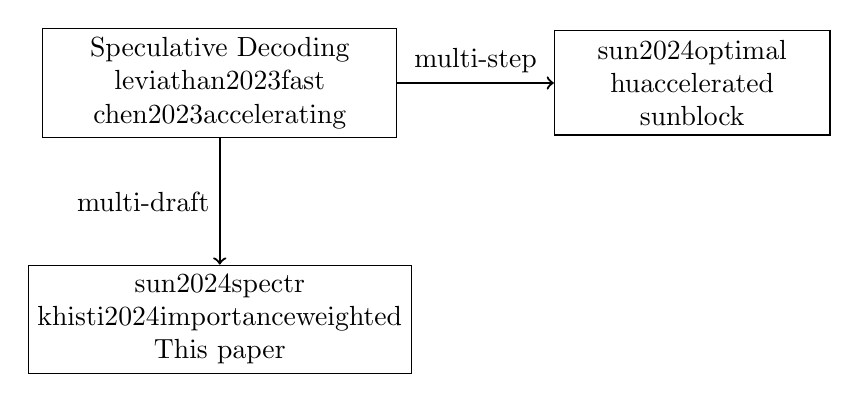
\begin{tikzpicture}[
    box/.style={draw, rectangle, minimum width=4.5cm, minimum height=1.2cm, align=center},
    smallbox/.style={draw, rectangle, minimum width=3.5cm, minimum height=1.2cm, align=center},
    arrow/.style={->, thick},
]

\node[box] (base) at (0,0) {Speculative Decoding \\ \citet{leviathan2023fast} \\ \citet{chen2023accelerating}};

\node[smallbox] (ms1) at (6,0) {\citet{sun2024optimal} \\ \citet{huaccelerated} \\ \citet{sunblock}};

\node[box] (md1) at (0,-3) {\citet{sun2024spectr} \\ \citet{khisti2024importanceweighted} \\ This paper};



\draw[arrow] (base) -- node[above] {multi-step} (ms1);
\draw[arrow] (base) -- node[left] {multi-draft} (md1);


\end{tikzpicture}

\caption{Different directions for improving speculative decoding.}
\label{fig:related_work}
\end{figure}


Multi-step speculative decoding and multi-draft speculative decoding represent different directions for improvement.

As shown in \Cref{fig:related_work}, \citet{sun2024spectr,khisti2024importanceweighted} and our work improve speculative decoding from the multi-draft perspective. When there is only a single draft, it reduces to the case in \citet{leviathan2023fast,chen2023accelerating}. On the other hand, \citet{sun2024optimal,huaccelerated,sunblock} enhance speculative decoding from the multi-step perspective. When there is only a single step, it reduces to the case in \citet{leviathan2023fast,chen2023accelerating}.

Combining both improvements in the multi-draft and multi-step scenario would be ideal, and could be a direction for future research.